\documentclass[10pt]{article}

% \usepackage{times}
\usepackage{amsmath}
\usepackage{amssymb}

\usepackage{amsthm}
\theoremstyle{plain}
\newtheorem{definition}{Definition}
\newtheorem{corollary}{Corollary}
\newtheorem{proposition}{Proposition}
\newtheorem{lemma}{Lemma}

\usepackage{txfonts}

\usepackage[en-GB]{datetime2}
\DTMlangsetup[en-GB]{ord=omit}

\usepackage{url}
\urlstyle{rm}

\usepackage[ruled,vlined,linesnumbered]{algorithm2e}
\SetKwFor{ForEach}{for each}{do}{end}
\SetKwProg{Function}{function}{}{}
\SetKwProg{Procedure}{procedure}{}{}
\SetKwProg{Class}{class}{}{}
\SetKwInput{Persistent}{persistent}{}{}
\SetKwInput{Input}{input}{}{}
\SetKwIF{WithProbability}{}{Else}{with probability}{do}{}{else}{end with}
\SetKw{Break}{break}
\DontPrintSemicolon

\usepackage{graphicx}

\usepackage{bm}
\newcommand{\vect}[1]{\bm{#1}}

\usepackage{forest}
\usepackage{tikz}
\usepackage{subcaption}

\DeclareMathOperator*{\argmax}{\arg\!\max}
\DeclareMathOperator*{\atantwo}{atan2}

\usepackage{mdframed}
\usepackage{xcolor}
\newenvironment{note}[1][Note]{
    \begin{center}
    	\begin{minipage}{0.9\linewidth}
    		\begin{mdframed}[backgroundcolor=yellow!25,linewidth=0pt]
    			\textbf{#1:} }{
    		\end{mdframed}
    	\end{minipage}
    \end{center}
}

\usepackage{booktabs}

\usepackage{pifont}
\newcommand{\cmark}{\ding{51}}
\newcommand{\xmark}{\ding{55}}

\usepackage{tikz}
\usetikzlibrary{calc}

\DeclareFontFamily{U}{mathx}{\hyphenchar\font45}
\DeclareFontShape{U}{mathx}{m}{n}{<5> <6> <7> <8> <9> <10> <10.95> <12> <14.4> <17.28> <20.74> <24.88> mathx10}{}
\DeclareSymbolFont{mathx}{U}{mathx}{m}{n}
\DeclareMathSymbol{\bigtimes}{1}{mathx}{"91}

\title{Simulator-Based Verification of Autonomous Vehicles: Agent-Based Test Generation}
\author{}
\date{\DTMcurrenttime, \today}

\begin{document}

\maketitle

\section{Introduction}

\begin{itemize}
    \item \textbf{Time} is implicit and discrete, with agents choosing actions at each timestep, and a time resolution constant specifying the simulation time between timesteps
    \item \textbf{State space} is continuous and feature-based techniques are probably more effective than discretisation
    \item \textbf{Actions} may be multi-body and/or multi-effector
    \item \textbf{Action space} is continuous and discretisation typically requires durative actions
    \item \textbf{Observability} is full, meaning that a sensor model is not required (although partial observability can be simulated)
    \item \textbf{Objectives} are goals states with transition costs/rewards, meaning in general that the horizon is indefinite, but a finite-horizon may also be imposed
    \item \textbf{Model} for transitions and objectives is unknown, but can be sampled through interaction with a simulator
    \item \textbf{Game} involving two or more players (agents), including a potentially adversarial design under verficiation (i.e.\ the ego agent)
    \item \textbf{Test generation} may be online (providing incomplete tests) or offline (providing complete tests)
\end{itemize}

\begin{note}
    Ideally a test should specify the optimal effector-actions to execute in a given state with respect to some test objective.
    A complete test then would be one that specifies effector-actions to execute in every reachable state.
    Online testing cannot guarantee complete tests because effector-actions are only determined for states that are actually encountered in a given run, and this does not typically cover all reachable states.
    For example, if a simulation involves non-deterministic action-selection, non-deterministic action-effects, or exogenous events, then these sources of uncertainty mean that a single execution of online testing will only reveal one of many possible runs.
    It may be possible to impose restrictions on a simulation so as to avoid many of these sources of uncertainty, but the actions of the ego agent remain uncontrollable.
    For example, a test may be complete for a given ego policy, but may be incomplete when faced with a different ego policy (since that policy may cause the system to transition into a state that was not accounted for in the original test).
    It follows that a test is only complete if it accounts for every source of uncertainty and also works for every possible ego policy.
    This is a very strong requirement and is unlikely to be satisfiable in practice (e.g.\ if agents execute actions simultaneously, then the ego policy is a priori unknown).
    This seems to imply that the aim of our work is not \emph{test generation} but rather \emph{online testing with optional capturing of incomplete tests}: re-running such tests could be useful for repeatability, but test execution may fail, and there would be no guarantees that tests remain optimal with respect to their original test objectives.
\end{note}

\newpage
\section{Preliminaries}
We rely on some standard mathematical notation:
$v_{i}$ is an element of vector $\vect{v} = (v_{1}, \dots, v_{n})$ with $\vect{v}_{-i} = (v_{1}, \dots, v_{i-1}, v_{i+1}, \dots, v_ {n})$ the subvector of $\vect{v}$ excluding~$v_{i}$,
$|S|$ is the cardinality of set $S$,
$2^{S}$ is the powerset of $S$,
$\Delta(S)$ is the set of probability distributions over $S$,
$\mathbb{R}$ is the set of real numbers with $\mathbb{R}^{\ge 0}$ the subset of non-negative real numbers,
% $\mathbb{Z}^{\ge 0}$ is the set of non-negative integers,
and $\mathbb{N}$ is the set of natural numbers.
A function $f : X \to Y$ is a surjection if for each $y \in Y$ there exists some $x \in X$ such that $f(x) = y$.
Given a function $f : X \to Y$, the inverse image of function $f$ is a function $f_{B,N}^{-1} : Y \to 2^{X}$ defined for each $y \in Y$ as $f_{B,N}^{-1}(y) = \{ x \in X \mid f(x) = y \}$.

\subsection{Normal-Form Games}
An ($n$-player) normal-form game is a tuple $(N, A, \vect{u})$ where $N = \{ 1, \dots, n \}$ is a finite set of players, $A = A_{1} \times \dots \times A_{n}$ is a set of action profiles with $A_{i}$ the (possibly infinite) set of actions available to player $i \in N$, and $\vect{u} = (u_{1}, \dots, u_{n})$ is a profile of utility functions with $u_{i} : A \to \mathbb{R}$ the utility function for~$i$.
A (mixed) strategy for player $i \in N$ is a probability distribution $\psi \in \Delta(A_{i})$ with $\vect{\psi} \in \Delta(A_{1}) \times \dots \times \Delta(A_{n})$ a (mixed) strategy profile.
A strategy $\psi$ for player $i \in N$ is a pure strategy if $\psi(a) = 1$ for some $a \in A_{i}$.
A strategy profile $\vect{\psi}$ is a pure strategy profile if $\psi_{i}$ is a pure strategy for each $i \in N$.
For convenience, we may denote a pure strategy $\psi$ for player $i \in N$ directly by the action $a \in A_{i}$ such that $\psi(a) = 1$.
Likewise, we may denote a pure strategy profile $\vect{\psi}$ directly by the action profile $\vect{a} \in A$ such that $\psi_{i}(a_{i}) = 1$ for each player $i \in N$.
The expected utility of a strategy profile $\vect{\psi}$ is defined as:
\begin{equation*}
	u_{i}(\vect{\psi}) = \sum_{\vect{a} \in A} u_{i}(\vect{a}) \prod_{j \in N} \psi_{j}(a_{j})
\end{equation*}

In game theory, a solution concept is a prediction of how a game will be played.
Solution concepts are typically based on the idea that each player will try to maximise their expected utility under the assumption that other players will do the same.
A feasible deviation from strategy profile $\vect{\psi}$ by player $i \in N$ is a strategy profile $\vect{\psi'} = (\vect{\psi}_{-i}, \psi')$ where $\psi'$ is a strategy for $i$.
A strategy profile $\vect{\psi}$ is a Nash equilibrium if no player $i \in N$ has a feasible deviation $\vect{\psi'}$ from $\vect{\psi}$ such that $u_{i}(\vect{\psi'}) > u_{i}(\vect{\psi})$.
Every normal-form game with a finite set of action profiles is guaranteed to have at least one (not necessarily pure) Nash equilibrium~\cite{Nash:AM:1951}.
A Nash equilibrium is also guaranteed to exist for certain classes of normal-form game with an infinite set of action profiles~\cite{}.

\subsection{Markov Games}
A (fully observable) Markov game is a tuple $(N, S, A, T, \vect{R})$ where
$N = \{ 1, \dots, n \}$ is a finite set of players,
$S$ is a (possibly infinite) set of states,
$A = A_{1} \times \dots \times A_{n}$ is a set of action profiles with $A_{i}$ the (possibly infinite) set of actions available to player $i \in N$,
$T : S \times A \to \Delta(S)$ is a (stochastic) transition function, and
$\vect{R} = (R_{1}, \dots, R_{n})$ is a profile of reward functions with $R_{i} : S \times A \times S \to \mathbb{R}$ the reward function for player $i \in N$.
A Markov game is zero-sum if $\sum_{i \in N} R_{i}(s, \vect{a}, s') = 0$ for each $\vect{a} \in A$ and all $s, s' \in S$.

Markov games (also known as stochastic games~\cite{Shapley:PNAS:1953}) are composed of a sequence of normal-form games, called stage games, where players seek to optimise their return for the whole game rather than for individual stage games.
The current stage game is determined by the current state, and players transition between states by executing actions simultaneously.
The game is said to be fully observable because players are assumed to observe the current (shared) state at each decision step.
Let $T(s, \vect{a}, s')$ denote the probability of transitioning to state $s' \in S$ after executing action profile $\vect{a} \in A$ in state $s \in S$ according to probability distribution $T(s, \vect{a})$.
The probability of transitioning to state $s' \in S$ after executing strategy profile $\vect{\psi}$ in state $s \in S$ is:
\begin{equation*}
    T(s, \vect{\psi}, s') = \prod_{\vect{a} \in A} T(s, \vect{a}, s') \prod_{j \in N} \psi_{j}(a_{j})
\end{equation*}
The stage game for state $s \in S$ is a normal-form game $(N, A, \vect{u})$ where the utility function $u_{i}$ for player $i \in N$ is defined for each action profile $\vect{a} \in A$ as the immediate expected reward:
\begin{equation*}
    u_{i}(\vect{a}) = \sum_{s' \in S} T(s, \vect{a}, s') R_{i}(s, \vect{a}, s')
\end{equation*}
Markov games subsume numerous other frameworks, including repeated games when $|S| = 1$, and Markov decision processes (MDPs) when $|N| = 1$.

Solutions to Markov games are represented as functions, called policies, that map \emph{histories} to strategies.
An execution is a possibly infinite sequence of states and action profiles $(s_{1}, \vect{a}_{1}, s_{2}, \vect{a}_{2}, \dots)$.
A history of length $t$ is a finite execution $h_{t} = (s_{1},a_{1},$ $\dots, a_{t-1}, s_{t})$ ending in a state.
Let $H_{t}$ be the set of histories of length $t$ with $D = \{ 1, 2, \dots, t_{\max} \}$ the set of decision-steps up to horizon $t_{\max} \in \mathbb{N} \cup \{ \infty \}$ and $H = \{ h \in H_{t} \mid t \in D \}$ the set of histories up to $t_{\max}$.
A (stochastic or mixed) policy for player $i \in N$ is a function $\pi_{i} : H' \to \Delta(A_{i})$ where $H' \subseteq H$.
Let $\pi_{i}(h, a)$ denote the probability that player $i \in N$ should execute action $a \in A_{i}$ in history $h \in H'$ according to strategy $\pi_{i}(h)$.
A policy $\pi_{i}$ for player $i \in N$ is a complete policy if $H' = H$, otherwise $\pi_{i}$ is a partial policy.
A policy $\pi_{i}$ for player $i \in N$ is a deterministic (or pure) policy if $\pi_{i}(h, a) = 1$ for each $h \in H'$ and some $a \in A_{i}$.
For convenience, we may denote a deterministic policy $\pi_{i}$ for player $i \in N$ directly by a policy $\pi_{i}' : H' \to A$ where $\pi_{i}'(h) = a$ such that $\pi_{i}(h, a) = 1$.
A policy $\pi_{i}$ for player $i \in N$ is Markovian if $\pi_{i}(h_{t}) = \pi_{i}(h_{t'})$ for all $h_{t}, h_{t'} \in H'$ such that $t = t'$ and $s_{t} = s_{t'}$.
A Markovian policy for player $i \in N$ may be written as $\pi_{i} : X \to \Delta(A_{i})$ where $X \subseteq S \times D$.
A Markovian policy $\pi_{i}$ for player $i \in N$ is a stationary policy if $\pi_{i}(s, t) = \pi_{i}(s, t')$ for all $(s, t), (s, t') \in X$, otherwise $\pi_{i}$ is a non-stationary policy.
A stationary Markovian policy for player $i \in N$ may be written as $\pi_{i} : S' \to \Delta(A_{i})$ where $S' \subseteq S$.
A tuple $\vect{\pi} = \left( \pi_{1}, \dots, \pi_{n} \right)$ is a policy profile over $H' \subseteq H$ if $\pi_{i}$ is a policy over $H'$ for each $i \in N$.
The strategy profile for history $h \in H'$ according to policy profile $\vect{\pi}$ is $\vect{\pi}(h) = \left( \pi_{1}(h), \dots, \pi_{n}(h) \right)$.

Solutions are only well-defined for certain classes of Markov game.
Two common examples are finite-horizon Markov games and infinite-horizon (discounted reward) Markov games.
A finite-horizon Markov game is a tuple $(\Gamma, t_{\max})$ where $\Gamma$ is a Markov game and $t_{\max} \in \mathbb{N}$ is a horizon.
An infinite-horizon Markov game is a tuple $(\Gamma, \gamma)$ where $\Gamma$ is a Markov game and $\gamma \in [0, 1)$ is a discount fbody.
It is known that attention can be restricted to stationary Markovian policies in the case of infinite-horizon Markov games, and to non-stationary Markovian policies in the case of finite-horizon Markov games.
Unless stated otherwise, we will assume hereafter that all policies are either stationary or non-stationary Markovian policies.
For an infinite-horizon Markov game $(\Gamma, \gamma)$, the expected value of policy profile $\vect{\pi}$ for player $i \in N$ in state $s \in S$ is:
\begin{equation*}
    V_{i}(\vect{\pi}, s) = \sum_{s' \in S} T(s, \vect{\pi}(s), s') \left[ R_{i}(s, \vect{\pi}(s), s') + \gamma V_{i}(\vect{\pi}, s') \right]
\end{equation*}
For a finite-horizon Markov game $(\Gamma, t_{\max})$, the expected value of policy profile $\vect{\pi}$ for player $i \in N$ in state $s \in S$, with $t \in D \cup \{ 0 \}$ remaining decision-steps, is:
\begin{align*}
    V_{i}(\vect{\pi}, s, t) =
    \begin{cases}
        \sum\limits_{s' \in S} T(s, \vect{\pi}(s, t), s') \left[ R_{i}(s, \vect{\pi}(s, t), s') + V_{i}(\vect{\pi}, s', t-1) \right] & \text{if $t > 0$} \\
        0 & \text{if $t = 0$}
    \end{cases}
\end{align*}
A feasible deviation from policy profile $\vect{\pi}$ by player $i \in N$ is a policy profile $\vect{\pi'} = (\vect{\pi}_{-i}, \pi')$ where $\pi'$ is a policy for $i$.
A policy profile $\vect{\pi}$ is a Nash equilibrium if no player $i \in N$ has a feasible deviation $\vect{\pi'}$ from $\vect{\pi}$ such that $V_{i}(\vect{\pi'}, h) \ge V_{i}(\vect{\pi}, h)$ for each $h \in H'$ and $V_{i}(\vect{\pi'}, h') > V_{i}(\vect{\pi}, h')$ for some $h' \in H'$.

\begin{note}[To do]
    Confirm that this definition of a Nash equilibrium is correct with respect to histories (or states, or time-indexed states).
\end{note}

\subsection{Stochastic Shortest Path Games}
A (fully observable) stochastic shortest path (SSP) game is a tuple $(N, S, A, T, \vect{C}, G)$ where
$N = \{ 1, \dots, n \}$ is a finite set of players,
$S$ is a (possibly infinite) set of states,
$A = A_{1} \times \dots \times A_{n}$ is a set of action profiles with $A_{i}$ the (possibly infinite) set of actions available to player $i \in N$,
$T : S \times A \to \Delta(S)$ is a (stochastic) transition function,
$\vect{C} = (C_{1}, \dots, C_{n})$ is a profile of cost functions with $C_{i} : S \times A \times S \to \mathbb{R}^{\ge 0}$ the (non-negative) cost function for player $i \in N$,
and $G = G_{1} \cup \dots \cup G_{n}$ is a non-empty set of goal states with $G_{i} \subseteq S$ the (possibly empty, possibly infinite) set of goal states for player $i \in N$.
Moreover, each cost function $C_{i}$ should satisfy $C_{i}(s, a, s') = 0$ if $s \in G$, or $C_{i}(s, a, s') > 0$ otherwise, for all $s, s' \in S$ and each $a \in A$.
Similarly, the transition function $T$ should satisfy $T(s, a, s) = 1$ for all $s \in G$ and each $a \in A$.
SSP games subsume numerous other frameworks, including finite- and infinite-horizon Markov games as well as SSP MDPs (which in turn subsume finite- and infinite-horizon MDPs as well as classical planning)~\cite{Bertsekas:book:1995,Patek:PhD:1997,Patek:JCO:1999,Kolobov:book:2012}.

\begin{note}
    I have only found definitions of $2$-player zero-sum SSP games in the literature, so this definition of an $n$-player general-sum SSP game is only an informed guess.
    The definition says that all players should seek to minimize their cost for the duration of the game, as is the case in Markov games, but that at least one player should seek to arrive in a goal state where the game will terminate.
    The definition does not explicitly capture the notion that an adversary would seek to block the goal-directed player from achieving their goal, but the fact that this notion appears in existing definitions may be due to those definitions focusing on zero-sum games.
\end{note}

\newpage
\section{Framework}\label{section:framework}

\begin{definition}\label{definition:model}
    An agent-body-effector model is a tuple $(N, B, E, f_{B,N}, f_{E,B})$ where:
    \begin{itemize}
        \item $N = \{ 1, \dots, n \}$ is a finite set of agents
        \item $B$ is a finite set of bodies with $f_{B,N} : B \to N$ a surjection from bodies to agents
        \item $E$ is a finite set of effectors with $f_{E,B} : E \to B$ a surjection from effectors to bodies and $A(e)$ the non-empty (possibly infinite) set of actions available to $e \in E$
    \end{itemize}
\end{definition}

\begin{corollary}
    $2 \le |N| \le |B| \le |E|$.
\end{corollary}

\begin{figure}[tbhp]
    \centering
    \scriptsize
    \begin{forest}
        for tree={s sep=-1pt},
        if level=0{l sep+=10pt}{},
        [MAS
            [Agent, label={above left:\emph{Design under Test}}
                [Body [Effector] [$\dots$] [Effector]]
                [$\dots$ [$\dots$]]
                [Body [Effector] [$\dots$] [Effector]]
            ]
            [$\dots$
                [$\dots$ [$\dots$]]
            ]
            [Agent, label={above right:\emph{Test Generator}}
                [Body [Effector] [$\dots$] [Effector]]
                [$\dots$ [$\dots$]]
                [Body [Effector] [$\dots$] [Effector, edge label={node[midway,above right]{\emph{Simulator}}}]]
            ]
        ]
        \draw (-5.25, -0.25) [dotted] rectangle (-2, -1.2);
        \draw (-0.5, -0.25) [dotted] rectangle (4.9, -1.2);
        \draw (-5.75, -1.3) [dotted] rectangle (6, -2.5);
    \end{forest}
    \caption{Agent-body-effector model}
    \label{figure:model}
\end{figure}

The set of bodies associated with agents $N' \subseteq N$ is defined as $B(N') = \{ b \in f_{B,N}^{-1}(i) \mid i \in N' \}$.
The set of effectors associated with bodies $B' \subseteq B$ is defined as $E(B') = \{ e \in f_{E,B}^{-1}(b) \mid b \in B' \}$.
Thus, the set of bodies $B$ (resp.\ agents $N$) in an agent-body-effector model induces a partition of the set of effectors $E$, as illustrated in Figure~\ref{figure:model}.
The set of (multi-)actions available to effectors $E' \subseteq E$ is defined as $A(E') = \bigtimes_{e \in E'} A(e)$.
Thus, there exists a non-empty set of (multi-)actions available to each body (resp.\ agent).

% \begin{definition}
%     A test generation game $(G, S, A, T, \vect{R})$ is collaborative if $R_{i}(s) = R_{j}(s)$ for all $i, j \in N \setminus \{ 1 \}$ and each $s \in S$.
% \end{definition}
%
% Simulator-based test generation constitutes a multi-agent system because it involves a group of (one or more) tester agents playing against a single ego agent: the former is under the control of the test generation system, while the latter is not.
% The objective of simulator-based test generation is then to design a group of tester agents so as to influence the ego agent towards achieving some test goal.
% Definition~\ref{definition:game} formally models this problem as a Markov game.
% Markov games assume that time is composed of discrete decision steps in which agents execute actions simultaneously.
% Although the transition function $T$ and reward functions $\vect{R}$ are specified in Definition~\ref{definition:game}, these may be unknown in practice (as is the case in multi-agent reinforcement learning).
% What is important is that a simulator provides feedback to agents in a way that constitutes sampling from $T$ and $\vect{R}$, allowing agents to approximate $T$ and $\vect{R}$ through interaction with the simulator.

\begin{definition}\label{definition:game}
    Let $(N, B, E, f_{B,N}, f_{E,B})$ be an agent-body-effector model.
    A stochastic shortest path game $(N, S, A, T, \vect{C}, G)$ is a simulator-based testing game if:
    \begin{itemize}
        \item $N = \{ 1, \dots, n \}$ such that $n \ge 2$ with $1$ the ego agent and $2, \dots, n$ the tester agents
        \item $A_{i} = A(E(B(\{ i \})))$ is the set of actions available to agent $i \in N$
    \end{itemize}
\end{definition}

\begin{note}[To do]
    Formally define the notion of proper policies.
\end{note}

\begin{lemma}\label{lemma:dead_ends}
    Let $\mathcal{G}$ be a simulator-based testing game.
    There exists a proper policy profile for $\mathcal{G}$ if and only if $\mathcal{G}$ does not exhibit dead-ends.
\end{lemma}

\begin{proof}[Proof Sketch]
    The proof may be analogous to the proofs for SSP MDPs~\cite{Kolobov:book:2012}, assuming it has not been proven already.
\end{proof}

\begin{definition}
    A time-limited test generation game is a tuple $(\mathcal{G}, t_{\max})$ where $\mathcal{G}$ is a test generation game and $t_{\max} \in \mathbb{N}$ is a (finite-)horizon.
\end{definition}

\begin{proposition}
    Let $(\mathcal{G}, t_{\max})$ be a time-limited test generation game.
    There exists a proper policy profile for $(\mathcal{G}, t_{\max})$.
\end{proposition}

\begin{proof}[Proof Sketch]
    The set of states $S$ can be translated into a new set of states $S' = S \times \{ 0, \dots, t_{\max} \}$.
    The set of goal states $G$ can be translated into a new set of goal states $G' = \left( G \times \{ 0, \dots, t_{\max} \} \right) \cup \left( S \times \{ 0 \} \right)$.
    The translated game $(\mathcal{G}', t_{\max})$ does not exhibit dead-ends because for any state $s \in S'$ there always exists a state $s' \in S \times \{ 0 \}$ such that $s'$ is reachable from $s$.
    Thus, it follows from Lemma~\ref{lemma:dead_ends} that a proper policy profile for $G$ is guaranteed to exist.
\end{proof}

% \begin{definition}
%     Let $\pi_{1}$ be a deterministic policy and $\omega \subseteq S$ be a (test) assertion.
%     An interesting test given $\pi_{1}$ and $\omega$ is a tuple $(s_{1}, \vect{\pi}_{-1})$ where $s_{1} \in S$ is an initial state and $\vect{\pi}_{-1}$ is a deterministic policy profile for the set of agents $N \setminus \{ 1 \}$ such that executing policy profile $(\pi_{1}, \vect{\pi}_{-1})$ in state $s_{1}$ leads to some state $s \in \omega$ within a finite number of timesteps.
% \end{definition}
%
% \begin{note}
%     Assertions could be generalised to sequences of states (e.g.\ using a termporal logic?) or to executions (e.g.\ with actions as events?).
% \end{note}
%
% \begin{note}
%     We assume that a stochastic policy is always fixed to a deterministic policy by controlling the seed, but this means the test is only interesting with respect to that seed.
%     Is there a more general notion?
% \end{note}
%
% \begin{note}
%     How to \emph{repeat} a test when a different ego policy $\pi_{1}'$ may cause the assertion to be avoided altogether (e.g.\ by causing the agents to arrive in history $h \in H$ such that $\vect{\pi}_{-1}$ is undefined for $h$)?
% \end{note}
%
% \begin{definition}
%     Let $\pi_{1}$ be an ego policy, $\omega \subseteq S$ be a (test) goal, and $\theta \in (0, 1]$ be a probability threshold.
%     A satisficing test for $\pi_{1}$ with respect to $\omega$ is a tuple $(s_{1}, \vect{\pi}_{-1})$ where $s_{1} \in S$ is an initial state and $\vect{\pi}_{-1}$ is a deterministic policy profile for the set of agents $N \setminus \{ 1 \}$ such that executing policy profile $(\pi_{1}, \vect{\pi}_{-1})$ in state $s_{1}$ guarantees termination in some state $s \in \omega$ with probability $p \ge \theta$.
% \end{definition}
%
% \begin{note}
%     Do we need a reward function $R : S \times A \times S \to \mathbb{R}$ (where the objective is to maximise expected reward) or a non-negative cost function $C : S \times A \times S \to \mathbb{R}^{\ge 0}$ (where the objective is to minimise expected cost)?
%     Goal-oriented MDPs are typically defined with the latter.
% \end{note}
%
% \begin{note}
%     What is the appropriate (or required) domain of the reward function?
%     For example:
%     \begin{itemize}
%         \item $R' : S \times A \to \mathbb{R}$ such that $R'(s, a) = R(s, a, s') = R(s, a, s'')$ for all $s', s'' \in S$
%         \item $R' : S \to \mathbb{R}$ such that $R'(s) = R(s', a, s) = R(s'', a', s)$ for all $s', s'' \in S$ and all $a, a' \in A$
%     \end{itemize}
% \end{note}
%
% \begin{note}
%     Do we need a horizon $t_{\max} \in \mathbb{N}$ and/or discount fbody $\gamma \in [0, 1)$?
%     For example:
%     \begin{itemize}
%         \item Finite-horizon Markov game with terminal states (horizon, terminal states, optional discount fbody)
%         \item Infinite-horizon Markov game with terminal states (discount fbody, terminal states, no horizon)
%         \item Indefinite-horizon Markov game (terminal states, no horizon, no discount fbody)
%     \end{itemize}
%     How to ensure early terminations are preferred (i.e.\ that longer runs do not have the opportunity to acrue more value)? How to guarantee that proper policies exist?
% \end{note}
%
% \begin{table}[htbp]
%     \footnotesize
%     \centering
%     \caption{MDP Comparison}
%     \begin{tabular}{c c c l}
%         \toprule
%         $t_{\max} \in \mathbb{N}$ & $\gamma \in [0, 1)$ & $G \subseteq S$ & Class \\
%         \midrule
%         \xmark & \xmark & \xmark & --- \\
%         \xmark & \xmark & \cmark & Stochastic shortest path (SSP) \\
%         \xmark & \cmark & \xmark & Infinite-horizon (IFH) $\subset$ SSP \\
%         \xmark & \cmark & \cmark & \emph{IFH with absorbing states $\subset$ IFH} \\
%         \cmark & \xmark & \xmark & Finite-horizon (FH) $\subset$ SSP \\
%         \cmark & \xmark & \cmark & \emph{FH with absorbing states $\subset$ FH?} \\
%         \cmark & \cmark & \xmark & \emph{FH with decaying rewards $\subset$ FH?} \\
%         \cmark & \cmark & \cmark & \emph{FH with absorbing states and decaying rewards $\subset$ FH?} \\
%         \bottomrule
%     \end{tabular}
% \end{table}
%
% \begin{note}
%     How should time limits in RL-style episodes be interpreted?
%     Do they correspond to a finite-horizon or are they just a training mechanism~\cite{Pardo:ICML:2018}?
% \end{note}

\newpage
\section{Experiments}\label{section:case-study}

\begin{figure}[tbph]
    \scriptsize
    \begin{subfigure}{\linewidth}
        \centering
        \begin{forest}
            for tree={s sep=-1pt},
            if level=0{l sep+=10pt}{},
            [MAS
                [AV, label={above left:\emph{Design under Test}}
                    [Vehicle [Acceleration] [Steering]]
                ]
                [Agent
                    [Pedestrian [Acceleration] [Steering]]
                ]
                [$\dots$
                    [$\dots$ [$\dots$]]
                ]
                [Agent, label={above right:\emph{Test Generator}}
                    [Pedestrian [Acceleration] [Steering, edge label={node[midway,above right]{~~~~~\emph{Simulator}}}]]
                ]
            ]
            \draw (-4.9, -0.25) [dotted] rectangle (-2, -1.2);
            \draw (-0.75, -0.25) [dotted] rectangle (4.6, -1.2);
            \draw (-4, -1.3) [dotted] rectangle (4.4, -2.5);
        \end{forest}
        \caption{single-body ego agent, $n$ single-body tester agents}
    \end{subfigure}
    \begin{subfigure}{\linewidth}
        \centering
        \begin{forest}
            for tree={s sep=-1pt},
            if level=0{l sep+=10pt}{},
            [MAS
                [AV, label={above left:\emph{Design under Test}}
                    [Vehicle [Acceleration] [Steering]]
                ]
                [Agent, label={above right:\emph{Test Generator}}
                    [Pedestrian [Acceleration] [Steering]]
                    [$\dots$ [$\dots$]]
                    [Pedestrian [Acceleration] [Steering, edge label={node[midway,above right]{~~~~~\emph{Simulator}}}]]
                ]
            ]
            \draw (-4.15, -0.25) [dotted] rectangle (-1.25, -1.2);
            \draw (1, -0.25) [dotted] rectangle (3.85, -1.2);
            \draw (-3.3, -1.3) [dotted] rectangle (5.15, -2.5);
        \end{forest}
        \caption{single-body ego agent, $1$ multi-body tester agent}
    \end{subfigure}
    \caption{Agent-based test generation in \textsc{CAV-Gym:Pedestrians}}
\end{figure}

\begin{figure}[htbp]
    \centering
    \frame{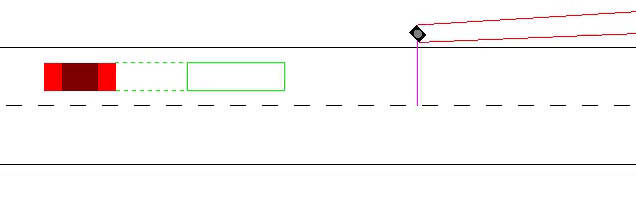
\includegraphics[width=\textwidth]{figures/cav-gym-cropped}}
    \caption{\textsc{CAV-Gym:Pedestrians}}
    \label{figure:cav-gym}
\end{figure}

\newpage
\bibliographystyle{plain}
\bibliography{agent-test-generation}

\newpage
\section*{Appendix: Kinematics}
A state is a tuple $s_{i} = (p_{i}, v_{i}, o_{i})$ where
$p_{i} \in \mathbb{R}^{2}$ is a position denoted $p_{i} = (p_{i}^{x}, p_{i}^{y})$,
$v_{i} \in [v_{\min}, v_{\max}]$ is a velocity with $v_{\min}, v_{\max} \in \mathbb{R}^{\ge 0}$ such that $v_{\min} < v_{\max}$,
and $o_{i} \in (-\pi, \pi]$ is an orientation (in radians).
Let $b \in \mathbb{R}^{\ge 0}$ be a wheelbase constant.
The positions of front and rear wheels $f_{i}, r_{i} \in \mathbb{R}^{2}$ in state $s_{i} = (p_{i}, v_{i}, o_{i})$ are:
\begin{align}
    f_{i} & = \left( p_{i} + \frac{b}{2} \cdot (\cos{o_{i}}, \sin{o_{i}}) \right) \\
    r_{i} & = \left( p_{i} - \frac{b}{2} \cdot \left( \cos{o_{i}}, \sin{o_{i}} \right) \right)
\end{align}
A body has two effectors: throttle and steering.
An action is a tuple $a_{i} = (t_{i}, e_{i})$ where
$t_{i} \in [t_{\min}, t_{\max}]$ is a throttle with $t_{\min}, t_{\max} \in \mathbb{R}$ such that $t_{\min} < t_{\max}$,
and $e_{i} \in (e_{\min}, e_{\max}]$ is a steering angle (in radians) with $e_{\min}, e_{\max} \in (-\pi, \pi]$ such that $e_{\min} < e_{\max}$.
Let $\lambda \in \mathbb{R}^{> 0}$ be a time resolution constant.
If action $a_{i} = (t_{i}, e_{i})$ is executed in state $s_{i} = (p_{i}, v_{i}, o_{i})$, then the successor state is $s_{i+1} = (p_{i+1}, v_{i+1}, o_{i+1})$ where:
\begin{align}
    f_{i+1} & = f_{i} + \left( v_{i} \cdot \lambda \cdot \left( \cos{o_{i} + e_{i}}, \sin{o_{i} + e_{i}} \right) \right) \\
    r_{i+1} & = r_{i} + \left( v_{i} \cdot \lambda \cdot \left( \cos{o_{i}}, \sin{o_{i}} \right) \right) \\
    p_{i+1} & = \frac{f_{i+1} + r_{i+1}}{2}  \\
    v_{i+1} & = \max{ \left\{ v_{\min}, \min{ \left\{ v_{\max}, v_{i} + \left( \lambda \cdot t_{i} \right) \right\} } \right\} } \\
    o_{i+1} & = \atantwo{ \left( f_{i+1}^{y} - r_{i+1}^{y}, f_{i+1}^{x} - r_{i+1}^{x} \right) }
\end{align}
The body kinematics from Equations 1--7 are illustrated in Figure~\ref{figure:kinematics}.

\begin{figure}[htbp]
    \centering
    \footnotesize
    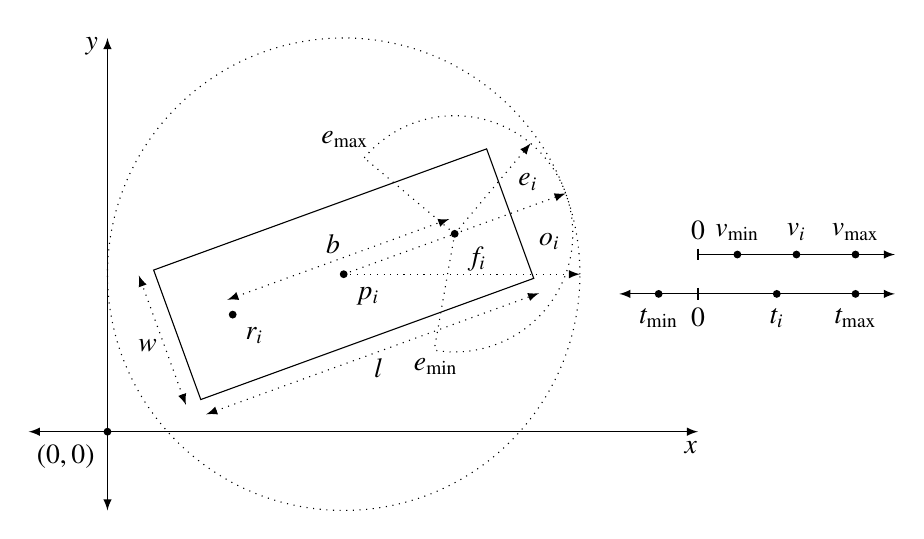
\begin{tikzpicture}
        \draw [latex-latex] (-1.0, 0.0) -- (7.5, 0.0); % X axis
        \draw [latex-latex] (0.0, -1.0) -- (0.0, 5.0); % Y axis
        \node at (7.4, -0.2) {$x$};
        \node at (-0.2, 4.9) {$y$};
        \node [circle, fill, inner sep=1pt, label={below left:$(0, 0)$}] at (0.0, 0.0) {};
        \draw [dotted] (3.0, 2.0) circle (3.0); % outer circle
        \draw [-latex, dotted] (3.0, 2.0) -- (6.0, 2.0); % outer circle, 0 degrees

        \begin{scope}[shift={(3.0, 2.0)}, rotate around={20.0:(0.0, 0.0)}]
            \draw (-2.25, -0.875) rectangle ++(4.5, 1.75);  % bounding box
            \node [circle, fill, inner sep=1pt, label={below right:$p_{i}$}] at (0.0, 0.0) {};
            \node [circle, fill, inner sep=1pt, label={below right:$f_{i}$}] at (1.5, 0.0) {};
            \node [circle, fill, inner sep=1pt, label={below right:$r_{i}$}] at (-1.5, 0.0) {};
            \draw [dotted] (0.0, 0.0) -- (1.5, 0.0); % outer circle, 20 degrees
            \draw [latex-latex, dotted] (-1.5, 0.2) -- (1.5, 0.2); % b arrow
            \node at (0.0, 0.4) {$b$};
            \draw [latex-latex, dotted] (-2.25, -1.075) -- (2.25, -1.075); % l arrow
            \node at (0.0, -1.275) {$l$};
            \draw [latex-latex, dotted] (-2.45, -0.875) -- (-2.45, 0.875); % w arrow
            \node at (-2.65, 0.0) {$w$};
            \node at (2.6, -0.5) {$o_{i}$};

            \begin{scope}[shift={(1.5, 0.0)}]  % inner circle
                \draw [dotted] (0.0, 0.0) ++(120:1.5) arc (120:-120:1.5); % inner circle
                \draw [-latex, dotted] (0.0, 0.0) -- (1.5, 0.0); % inner circle, 0 degrees
                \draw [-latex, dotted, rotate around={30.0:(0.0, 0.0)}] (0.0, 0.0) -- (1.5, 0.0); % inner circle, 30 degrees
                \draw [dotted, rotate around={120:(0.0, 0.0)}] (0.0, 0.0) -- (1.5, 0.0); % inner circle, left line
                \draw [dotted, rotate around={-120:(0.0, 0.0)}] (0.0, 0.0) -- (1.5, 0.0); % inner circle, right line
                \node at (1.1, 0.3) {$e_{i}$};
                \node at (-0.9, 1.6) {$e_{\max}$};
                \node at (-0.8, -1.5) {$e_{\min}$};
            \end{scope}
        \end{scope}

        \begin{scope}[shift={(6.5, 2.0)}]
            \begin{scope}[shift={(1.0, 0.25)}]
                \draw [-latex] (0.0, 0.0) -- (2.5, 0.0);
                \draw (0.0, 0.075) -- (0.0, -0.075);
                \node [circle, inner sep=1pt, label={above:$0$}] at (0.0, 0.0) {};
                \node [circle, fill, inner sep=1pt, label={above:$v_{\min}$}] at (0.5, 0.0) {};
                \node [circle, fill, inner sep=1pt, label={above:$v_{\max}$}] at (2.0, 0.0) {};
                \node [circle, fill, inner sep=1pt, label={above:$v_{i}$}] at (1.25, 0.0) {};
            \end{scope}
            \begin{scope}[shift={(0.0, -0.25)}]
                \draw [latex-latex] (0.0, 0.0) -- (3.5, 0.0);
                \draw (1.0, 0.075) -- (1.0, -0.075);
                \node [circle, inner sep=1pt, label={below:$0$}] at (1.0, 0.0) {};
                \node [circle, fill, inner sep=1pt, label={below:$t_{\min}$}] at (0.5, 0.0) {};
                \node [circle, fill, inner sep=1pt, label={below:$t_{\max}$}] at (3.0, 0.0) {};
                \node [circle, fill, inner sep=1pt, label={below:$t_{i}$}] at (2.0, 0.0) {};
            \end{scope}
        \end{scope}
    \end{tikzpicture}
    \caption{Body kinematics}
    \label{figure:kinematics}
\end{figure}

\begin{note}[Problem]
    Given state $s_{i}$ and target orientation $o_{g}$ such that $o_{g}$ is reachable from $s_{i}$ with a single action, find steering angle $e_{i}$ such that executing action $a_{i} = (t_{i}, e_{i})$ in $s_{i}$ results in successor state $s_{i+1} = (p_{i+1}, v_{i+1}, o_{i+1})$ where $o_{i+1} = o_{g}$ for any throttle $t_{i}$.
\end{note}

\newpage
\section*{Appendix: Algorithms}

\begin{note}[To do]
    Account for discretisation of continuous action spaces within each agent type (although, strictly speaking, \textsc{QLearningAgent} is the only agent type that requires a finite action space).
\end{note}

\begin{algorithm}[htbp]
	\caption{\textsc{Simulator}}
	\label{algorithm:simulation}
	\footnotesize
    \Persistent{environment $e$, agents $N = \{ 1, \dots, n \}$, terminator $\psi \subseteq S$}
    \Begin{
        \ForEach{episode}{
            $s \leftarrow$ reset $e$\;
            \ForEach{timestep}{
                $\vect{a} \leftarrow \left( \textsc{ChooseAction}_{1}(s), \dots, \textsc{ChooseAction}_{n}(s) \right)$\;
                $\vect{r}, s' \leftarrow$ execute $\vect{a}$ in $e$\;
                \ForEach{agent $i \in N$}{$\textsc{ProcessFeedback}_{i}(s, a_{i}, r_{i}, s')$}
                \leIf{$s' \in \psi$}{\Break}{$s \leftarrow s'$}
            }
        }
    }
\end{algorithm}

\begin{algorithm}[htbp]
	\caption{\textsc{RandomAgent}}
	\label{algorithm:random_agent}
	\footnotesize
    \Persistent{exploration rate $\epsilon \in [0, 1]$}
    \Function{$\textsc{ChooseAction}(s)$}{
        \WithProbability{$\epsilon$}{
            \Return random choice from $A(s)$
        }
        \Return $\varnothing$
    }
\end{algorithm}

\begin{algorithm}[htbp]
	\caption{\textsc{ProgrammedRandomAgent}}
	\label{algorithm:random_constrained_agent}
	\footnotesize
    \Persistent{programmed behaviour $\pi : S \to A$, terminator $\psi \subseteq S$, exploration rate $\epsilon \in [0, 1]$}
    \Function{$\textsc{ChooseAction}(s)$}{
        \If{$\pi$ is active}{
            \leIf{$s \in \psi$}{set $\pi$ as inactive}{\Return $\pi(s)$}
        }
        \WithProbability{$\epsilon$}{
            set $\pi$ as active\;
            \Return $\pi(s)$
        }
        \Return $\varnothing$
    }
\end{algorithm}

\begin{algorithm}[htbp]
	\caption{\textsc{ProgrammedReactiveAgent}}
	\label{algorithm:proximity_agent}
	\footnotesize
    \Persistent{programmed behaviour $\pi : S \to A$, trigger $\varphi \subseteq S$, terminator $\psi \subseteq S$}
    \Function{$\textsc{ChooseAction}(s)$}{
        \If{$\pi$ is active}{
            \leIf{$s \in \psi$}{set $\pi$ as inactive}{\Return $\pi(s)$}
        }
        \If{$s \in \varphi$}{
            set $\pi$ as active\;
            \Return $\pi(s)$
        }
        \Return $\varnothing$
    }
\end{algorithm}

\begin{algorithm}[htbp]
	\caption{\textsc{ProgrammedElectionAgent}}
	\label{algorithm:election_agent}
	\footnotesize
    \Persistent{programmed behaviour $\pi : S \to A$, terminator $\psi \subseteq S$, coordinator $c$}
    \Function{$\textsc{ChooseAction}(s)$}{
        \If{$\pi$ is active}{
            \leIf{$s \in \psi$}{set $\pi$ as inactive}{\Return $\pi(s)$}
        }
        \If{elected by $c$}{
            set $\pi$ as active\;
            \Return $\pi(s)$
        }
        \Return $\varnothing$
    }
\end{algorithm}

\begin{algorithm}[htbp]
	\caption{\textsc{QLearningAgent}}
	\label{algorithm:qlearning_agent}
	\footnotesize
    \Persistent{learning rate $\alpha \in [0, 1]$, discount fbody $\gamma \in [0, 1)$, exploration rate $\epsilon \in [0, 1]$,\newline
    feature $f_{j} : S \times A \to \mathbb{R}$ with weight $w_{j} \in \mathbb{R}$ for $j = 1, \dots, m$}
    \Function{$\textsc{ChooseAction}(s)$}{
        \WithProbability{$\epsilon$}{
            \Return random choice from $A(s)$
        }
        \Return random choice from $\argmax_{a \in A(s)} \textsc{QValue}(s, a)$
    }
    \Procedure{$\textsc{ProcessFeedback}(s, a, r, s')$}{
        $q \leftarrow \left( r + \gamma \cdot \max_{a' \in A(s')} \textsc{QValue}(s', a') \right) - \textsc{QValue}(s, a)$\;
        \ForEach{feature $f_{j}$}{$w_{j} \leftarrow w_{j} + \alpha \cdot q \cdot f_{j}(s, a)$}
    }
    \Function{$\textsc{QValue}(s, a)$}{
        \Return $\sum_{j = 1}^{m} f_{j}(s, a) \cdot w_{j}$
    }
\end{algorithm}

\end{document}
